% define document class and set class options
\documentclass[11pt, a4paper]{article}

%===============================================
% *** LIST OF GENERAL PACKAGES *** %
% language package (french option available as well)
\usepackage[english]{babel}

% input fonts
\usepackage[utf8]{inputenc}
\usepackage[T1]{fontenc}
\usepackage{csquotes}

% customize default page geometry (size of margins, ...)
\usepackage{geometry}
\geometry{hmargin=2cm,vmargin=3cm}
\usepackage{titling}

\usepackage{titlesec}

% writing style
\usepackage{lmodern}
\usepackage{times}	 

% include images (image extensions & paths)
\usepackage{graphicx}
\DeclareGraphicsExtensions{.pdf,.jpg,.png,.eps}
\graphicspath{{figs/}}

\usepackage{wrapfig}

% display hyperlinks in the text
\usepackage{hyperref}  %
\hypersetup{colorlinks,%
            citecolor=red,%
            filecolor=black,%
            linkcolor=blue,%
            urlcolor=blue,%
            breaklinks=true}
            
% customize enumerated lists
\usepackage{enumitem}

% lipsum command to fill in the document (for visualisation purposes)
\usepackage{lipsum}

%===============================================
% *** CAPTIONS AND SUBFIGURES *** %
\usepackage{subcaption}

%===============================================
% *** TABLES *** %
\usepackage{booktabs}
\usepackage{multirow}

%=============================================== 
% *** BIBLIOGRAPHY (FOR BIBLATEX) *** %
\usepackage[
    backend=biber,
    style=ieee,
    ]{biblatex}

\usepackage{bookmark}
\addbibresource{bgtg_lib.bib}

% citation style: apa, ieee, authoryear, ...

%===============================================
% *** MATHS / PHYSICS PACKAGES *** %
\usepackage{amsfonts,amssymb,amsmath,amsthm}
\usepackage{mathrsfs}
\usepackage{mathtools}  % for DeclarePairedDelimiter
\usepackage{siunitx}    % notation physical units

% notations (shortcuts)
\newcommand{\bs}[1]{\boldsymbol{#1}}
\newcommand{\nbpix}{N}
\DeclareMathOperator{\prox}{prox}
\DeclareMathOperator{\sgn}{sgn}
\DeclareMathOperator*{\argmin}{argmin}
\DeclarePairedDelimiter{\norm}{\lVert}{\rVert}

%===============================================
% *** TITLE, AUTHOR AND DATE *** %
% \pretitle{\begin{center}\fontsize{30bp}{30bp}\selectfont}
% \posttitle{\par\end{center}}

% \preauthor{\begin{center}\fontsize{14bp}{14bp}\selectfont}
% \postauthor{\par\end{center}}
%===============================================
% *** MAIN DOCUMENT *** %
\begin{document}

\begin{titlepage}
\centering
% Logos
\begin{minipage}{.25\linewidth}

\includegraphics[width=\linewidth]{../images-figures/ulille.png}
\end{minipage}
\hfill
\begin{minipage}{.25\linewidth}
\centering

\includegraphics[width=\linewidth]{../images-figures/Centrale-Lille-Ecole.png}
\end{minipage}
\hfill
\begin{minipage}{.25\linewidth}

\includegraphics[width=\linewidth]{../images-figures/imt.png}
\end{minipage}

\vfill

% Subtitle

{\large Research project final report \\ \textit{March 2025} \vspace{1\baselineskip}}

% Title
\begin{minipage}{\linewidth}
\huge
\bfseries
\centering
\rule{\linewidth}{1.5pt}\\
Conditional Generation of Bass Guitar Tablature for Guitar Accompaniment in Western Popular Music\\[-3mm]
\rule{\linewidth}{1.5pt}
\end{minipage}

\vfill

% Persons involved 
\begin{minipage}{.45\linewidth}
\textit{Student:}\\
Olivier \textsc{Anoufa}\\
\textit{Data Science Master 2}

\end{minipage}
\hfill
\begin{minipage}{.45\linewidth}
\flushright
\textit{Supervisors:}\\
Alexandre \textsc{D'Hooge}\\
Ken \textsc{Déguernel}\\
\textit{Algomus team, CRIStAL}
\end{minipage}

\vfill

% Abstract
\begin{flushleft}
\justify
\textbf{Abstract ---} The field of symbolic music generation has seen great advancements with the rise of transformer-based architectures.
Addressing a specific need identified through a user study conducted on guitar players, we focus on developing AI tools to generate bass guitar tablatures conditioned on scores of other instruments in Western popular music.
The bass guitar, a crucial component of the rhythmic and harmonic sections in music, presents a unique challenge due to its dual role in providing structure and groove.
Building upon the tablature notation, the most popular way to share music among guitarists, this work adopts modern encoding schemes to integrate tablature representation into transformer-based models.
To this end, the project involves preprocessing a large dataset of music scores and fine-tuning state-of-the-art transformer architectures.
Due to the project being the first of its kind and its creative nature, the evaluation of the generated tablatures is mainly done qualitatively.
\vspace{.5\baselineskip}\\
\end{flushleft}
\vfill


% Period
% October 1st --- March 31st
% \vspace{1\baselineskip}\\
\begin{flushleft}
\textbf{Key-words ---} music information retrieval, conditional generation, guitar accompaniment, bass guitar, tablature;
\vspace{.5\baselineskip}\\
% \textbf{Mots-clés \hspace{1ex}---} effets audio, traitement de l'information musicale, traitement du signal différentiable, reproduction sonore, musique assistée par ordinateur.
\end{flushleft}
\vfill

% More logos
\begin{minipage}{.25\linewidth}

\includegraphics[height=3cm]{../images-figures/logoCRIStAL.png}
\end{minipage}
\hspace{7cm}
\begin{minipage}{.25\linewidth}

\includegraphics[height=3cm]{../images-figures/cnrs.png}
\end{minipage}

\end{titlepage}


% \begin{figure}[t]% We use titling to put a figure on top of the title page
%     \centering
%     
\includegraphics[width=.5\linewidth]{logos_empile}
% \end{figure}

% \title{Bass guitar tablature conditional generation for guitar accompaniment in western popular music}

% \author{Olivier \textsc{Anoufa} \\  University of Lille, France \\ Master 2 Data Science: Research project}

% {\let\newpage\relax\maketitle}

\newpage

\section*{Introduction}

% Context and motivation
Natural language processing methods for the generation of symbolic music have experienced significant advancements in recent years.
The transformer architecture, introduced by Vaswani et al. in 2017, has been used to generate scores for various instruments, in diverse styles and genres\cite{vaswaniAttentionAllYou2023, leNaturalLanguageProcessing2024}.
An unpublished user study conducted by Bacot et al. showed a potential need for accompaniment generation tools for guitarists.
The questionnaire was answered by 31 guitarist-composers, and 7 of them followed up with an interview.
During the interviews, the focus was on generating bass guitar lines and drum parts without requiring familiarity with the instruments.
Indeed, guitarists often resort to writing basic bass lines to accompany their compositions, and an AI tool could perform this functional task for them\cite{bacot_tablature_2025}.

% Objectives
This need is the starting point for this project, proposed by the Algomus team, which is part of the CRIStAL laboratory.
In this project, we focus on the conditional aspect of symbolic music generation, for an instrument that has not been thoroughly studied yet: the bass guitar.
Specifically, the goal is to generate bass guitar tablatures given other instruments' scores, in the context of western popular music.
Our objective is to try several combinations of instruments and evaluate the quality of the generated tablatures both numerically and with the help of musicians.


% Terms definition (tablature, add the period when it was used)
% Difference between guitar and bass (role in the music)
To better understand what is at stake in this challenge, we will begin by precisely defining the role of the bass guitar in the context of western popular music.
Since the human ear perceives low-frequency pulses more distinctly, the bass guitar is considered part of the rhythmic section of the band (together with the drums)\cite{hoveSuperiorTimePerception2014}.
However, the bass guitar also performs a harmonic — and sometimes melodic — role in the music, sustaining the lead instruments and adding depth to the composition.
Its adaptability makes the bass guitar a vital component across various genres of western popular music.


Historically, tablatures have been used since the Renaissance period as a simplified notation system for string instruments like the lute.
Originating around the 16th century, tablatures were an intuitive alternative to staff notation, allowing musicians to bypass the complexity of interpreting pitches.
This system explicitly linked symbols to physical actions on the instrument, such as pressing specific frets or strings.
As a result, tablatures gained popularity among amateur and professional musicians alike.
In modern times, tools like GuitarPro have digitalized tablatures, further extending their use for learning, practice, and composition in genres ranging from classical to popular music\cite{sarmentoDadaGPDatasetTokenized2021}.

% add a fig Time is running out, melodic and rhythmic bass
\begin{figure}[h!]
    \centering
    \begin{minipage}{0.45\textwidth}
        \centering
        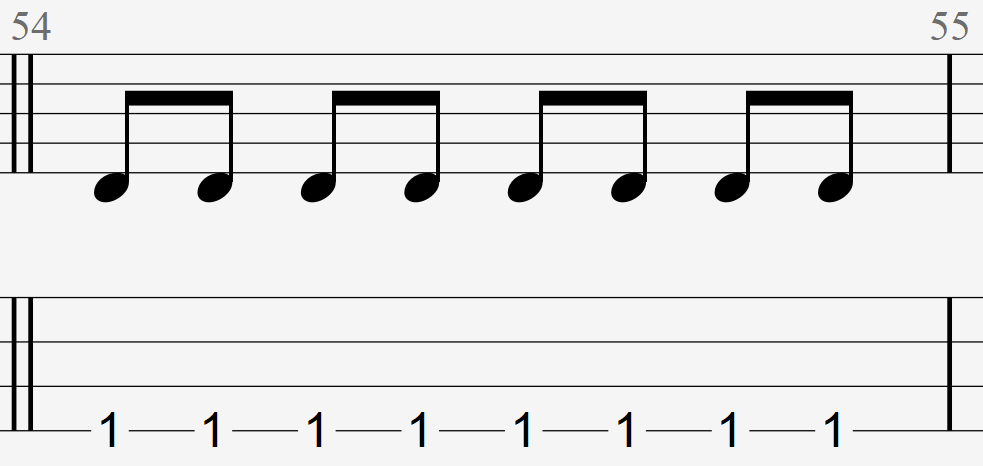
\includegraphics[width=.5\linewidth]{figs/rhythmic_tab_TIRO.png}
        \caption{Rhythmic extract}
    \end{minipage}%
    \hfill
    \begin{minipage}{0.45\textwidth}
        \centering
        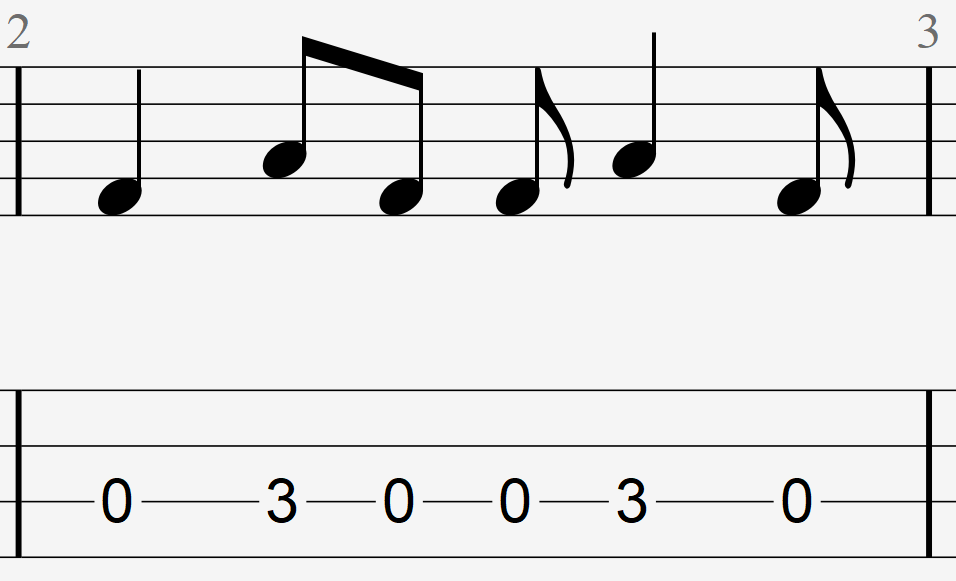
\includegraphics[width=.5\linewidth]{figs/melodic_tab_TIRO.png}
        \caption{Melodic extract}
    \end{minipage}
    \label{fig:bass_tab_TIRO}
    \caption{Rhythmic and melodic extracts in Time is Running Out by Muse}
\end{figure}


\ref{fig:bass_tab_TIRO} shows a tablature and score extract of both a rhythmic and a more melodic bass.
Scores display the notes to play, while tablatures show the fingering to use on the instrument.
More precisely, each line of the tablature represents a string of the instrument, and the numbers indicate the fret to press on the string.
For instance, in the figure on the right, the bassist will start by playing the fourth string with the first fret.
Tablatures do not contain rhythmic information, which is why they are generally combined with scores.
Otherwise, the musician must know the song to play it correctly.


% Abstract challenges: (high-level such as: propose an informatic representation of music...)
Generating bass guitar tablatures presents several challenges.
At a high level, we first need to scrape, preprocess, and curate large datasets of music scores.
Then, we need to design a computational representation of music that is adapted to the task of generating bass guitar tablatures.
That is, a way to encode music scores in a meaningful way for the transformer architecture we will use.
We will start by leveraging state-of-the-art models but will adapt and tune them to the task at hand.


\section*{State of the art}

% Challenges (tokenization, conditional generation, attention, data cleaning), training of the model)
Adapting the transformer architecture — originally developed for text processing — to symbolic music presents many challenges.
Symbolic music datasets, unlike text corpus, are limited in both size and diversity, posing challenges for training robust models\cite{leNaturalLanguageProcessing2024}.
Tokenization must be tailored to represent pitch, duration, and dynamics, while attention mechanisms require adaptation to capture the hierarchical and temporal structure of music.
Furthermore, data cleaning and preprocessing steps are critical to standardizing music scores and ensuring compatibility with sequence models.

% State of the art (survey, DadaGP, Compound Gen, Structure-informed positional encoding, gen coherent drum accompaniment)
% ResearchRabbit to find potential other articles

\subsection*{Data availability}


Symbolic music datasets are a cornerstone for training deep learning models, yet their availability and quality significantly vary across domains.
In music composition and generation, datasets are often limited in size and diversity, especially when compared to text or image datasets.
For bass guitar tablatures, the challenge is even more pronounced due to the niche nature of the instrument and the focus on other instruments in existing datasets.


The MIDI standard has dominated symbolic music datasets for decades, enabling the development of large-scale resources like the Lakh MIDI dataset and MAESTRO dataset.
However, while these datasets offer general-purpose symbolic music, they lack the specificity required for tasks involving tablatures or instrument-specific representation.
The GuitarSet dataset, for example, focuses on acoustic guitar transcription but does not provide sufficient symbolic information for bass guitar.
Similarly, the DadaGP dataset addresses the need for multi-instrument symbolic music data in tablature format, but its emphasis is on rock and metal genres, which limits the diversity of bass guitar styles\cite{sarmentoDadaGPDatasetTokenized2021}.


Bass guitar data, especially in tablature format, suffers from a lack of standardization and availability.
Tablature files are often stored in private formats like GuitarPro or as non-standardized text files, making it challenging to preprocess them for machine learning tasks\cite{sarmentoDadaGPDatasetTokenized2021}.
Moreover, rhythm and dynamics, critical elements in bass guitar playing, are frequently absent in publicly available tablatures, complicating their utility in generative tasks.


Efforts like DadaGP illustrate the potential for leveraging existing repositories of GuitarPro files to create symbolic datasets that include bass guitar parts.
Such datasets provide a tokenized format inspired by MIDI encodings, offering a foundation for training sequence models.
Additionally, pre-trained models on broader datasets like MAESTRO or Lakh MIDI can be fine-tuned on smaller datasets, reducing the dependency on large volumes of task-specific data\cite{makrisConditionalDrumsGeneration2022, sarmentoDadaGPDatasetTokenized2021}.
For our project, we use the DadaGP dataset. DadaGP comes with a very specific tokenization that we discuss in the next section.


\subsection*{Tokenization}

Tokenization in the context of deep learning music generation has been discussed by several previous works.
\cite{agarwalStructureinformedPositionalEncoding2024, makrisConditionalDrumsGeneration2022, sarmentoDadaGPDatasetTokenized2021, hsiaoCompoundWordTransformer2021, cournutEncodagesTablaturesPour2020}

% General overview of the possible startegies (NLP survey)
Tokenization in music involves converting complex musical content into a sequence of elements that can be processed computationally.
Much like tokenization in natural language processing (NLP), it breaks down music into manageable units, though in music, the focus is on musical features like pitch, duration, and velocity.
In symbolic music information retrieval (MIR), tokenization strategies are generally classified into two categories: time-slice-based and event-based. 
Time-slice-based tokenization divides music into fixed-time intervals, such as 16th notes, which can be represented in formats like piano rolls or multi-hot vectors, capturing simultaneous notes at each time slice.
Event-based tokenization, on the other hand, focuses on specific musical events, such as a note being played or a measure starting, often using formats like MIDI, which encode music as a series of events.
This approach can involve elementary tokens, which represent individual features like pitch or duration, or composite tokens that aggregate multiple features into one token, providing a more compact representation.
Notably, tokenization strategies like REMI (Revamped MIDI-derived events) and MIDI-like tokenization allow for consistent representation of rhythmic and pitch elements while addressing complexities like polyphony and multiple tracks in multi-instrument music\cite{leNaturalLanguageProcessing2024}.


% DadaGP tokenization
The DadaGP tokenization format adopts an event-based approach, similar to other music generation models, by representing musical events as discrete tokens.
It uses a Python script with PyGuitarPro to convert GuitarPro files into a tokenized sequence, beginning with metadata tokens such as artist, downtune, tempo, and start.
Pitched instrument notes are encoded with a combination of tokens representing instrument, note, string, and fret, while rests are denoted with a separate token structure.
For drumset sounds, a specific tokenization scheme using MIDI percussion maps is employed, where each drum sound is represented by a unique token (e.g., drums:note:36 for a kick drum).
The system also uses wait tokens to separate notes and rests, enabling the model to infer note durations without the need for explicit note-off tokens.
This approach ensures that new notes automatically silence previous ones, except in cases where ghost notes or let-ring effects are involved.
Additionally, the tokenization format records changes in musical structure, such as new measures, tempo shifts, and note effects, with each change being represented as a distinct token.
This flexible tokenization system allows for creative exploration, as it is resilient to syntax errors and can handle out-of-distribution sequences, making it particularly suitable for generative tasks.

\begin{figure}[h!]
    \centering
    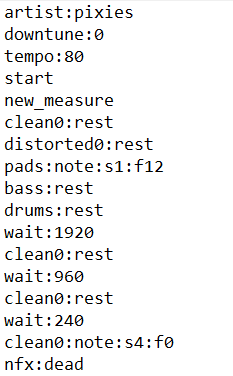
\includegraphics[width=.5\linewidth]{figs/dadagp_tokenization_pixies_wimm.png}
    \caption{First tokens of Where is my mind - Pixies}
    \label{fig:dadagp_tokenization}
\end{figure}


% Compound Gen tokenization



\subsection*{Conditional generation}

% What we have done (data preprocessing, getting the rhythmic instrument, retrieving the tokens, baseline using dadagp (GuitarCTRL))
% draw io fig of the model


% Workplan (what we are going to do)

\newpage

%\nocite{*} % force display of the full content of the .bib file, w/o any citation in the document
\printbibliography% references: print bibliography (with bibtex file)

\end{document}